%  FICHIER  :   template_fira_two_cols.tex
%  A copier à côté des autres .tex et à déclarer dans config.json
% ------------------------------------------------------------------
\documentclass[11pt,a4paper]{article}

% ─── pack de base ─────────────────────────────────────────────────
\usepackage[T1]{fontenc}
\usepackage[utf8]{inputenc}
\usepackage[british]{babel}
\usepackage[left=0mm,right=0mm,top=0mm,bottom=0mm]{geometry}
\usepackage[stretch=25,shrink=25,tracking=true,letterspace=30]{microtype}
\usepackage{graphicx,xcolor,marvosym,enumitem,paracol,hyperref}
\usepackage{FiraSans}
\renewcommand{\familydefault}{\sfdefault}
\usepackage{array} 
\usepackage{tabularx}
\usepackage{ragged2e}
 \usepackage{fontawesome}
% ─── couleurs & listes ────────────────────────────────────────────
\definecolor{cvblue}{HTML}{304263}
\setlist{parsep=0pt,topsep=0pt,partopsep=1pt,itemsep=1pt,leftmargin=6mm}
\hypersetup{colorlinks=true,urlcolor=white,linkcolor=white}

% ─── macros maison (identiques au modèle original) ────────────────
\newcommand{\dates}[1]{\hfill\textbf{#1}}
\newcommand{\is}{\par\vskip.5ex plus .4ex}
\newcommand{\smaller}[1]{{\small$\diamond$\ #1}}
\newcommand{\headleft}[1]{\vspace*{3ex}\textsc{\textbf{#1}}\par%
  \vspace*{-1.5ex}\hrulefill\par\vspace*{0.7ex}}
\newcommand{\headright}[1]{\vspace*{2.5ex}\textsc{\Large\color{cvblue}#1}\par%
  \vspace*{-2ex}{\color{cvblue}\hrulefill}\par}

% ─── défaut de secours si sidetext absent dans d’autres modèles ───
\providecolor{sidetext}{rgb}{0,0,0}
\definecolor{maincolor}{HTML}{ffffff}
% ─────────────────────────── DOCUMENT ─────────────────────────────
\begin{document}
\thispagestyle{empty}
\setlength{\topskip}{0pt}\setlength{\parindent}{0pt}\setlength{\parskip}{0pt}
\raggedbottom

\begin{minipage}[t]{0.33\textwidth}
  % Bande bleue d’en-tête
  \colorbox{cvblue}{\begin{minipage}[t][5mm][t]{\textwidth}\null\end{minipage}}
  \vspace{-.2ex}
  \colorbox{cvblue!90}{%
    \color{white}\kern0.09\textwidth
    \begin{minipage}[t][293mm][t]{0.82\textwidth}\raggedright
      \vspace*{2.5ex}
      % -------- Identité ------------------------------------------
      \Large Judikael MOUROUVIN\normalsize

      % Photo (s’affiche seulement si 8712cb35f7bf40ab87bae37c7d9a2c9d.png ≠ vide)
      \ifx\relax8712cb35f7bf40ab87bae37c7d9a2c9d.png\relax\else
        \vspace{2ex}\null\hfill
        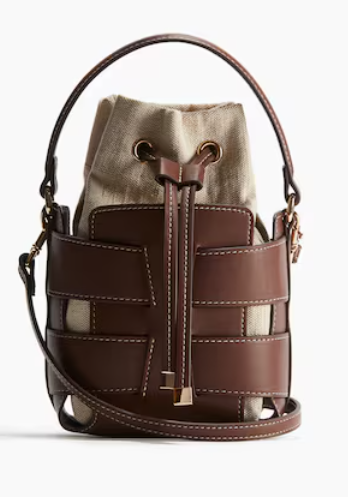
\includegraphics[width=0.65\textwidth]{8712cb35f7bf40ab87bae37c7d9a2c9d.png}
        \hfill\null
      \fi

      % -------- Profil -------------------------------------------
      \headleft{Profil}
      Passionné par l’informatique et le marketing digital, je maîtrise la configuration de postes, la maintenance et le diagnostic d’incidents. Mon année d’alternance à la DSI de la Mairie du Gosier m’a permis de gérer des projets numériques et de former des utilisateurs. Rigoureux et orienté résultats, je souhaite désormais mettre mes compétences au service de nouveaux défis à temps plein. Mon objectif est d’accompagner votre structure dans la mise en place de solutions fiables et performantes.

      % -------- Contact ------------------------------------------
      \headleft{Contact}\small
      \MVAt\  \texttt{jkmou971@gmail.com}\par
      \Mobilefone\ +590 0690 91 14 48\par
      \Letter\ Route de COCOYER\par
      97190 GOSIER\par
      \faLinkedin\  \href{}{}
      \normalsize

      % -------- Langues (si dispo) -------------------------------
      \ifx\relax\begin{itemize}[leftmargin=*]
\item English - \textcolor{gray}{}
\item Espagnol - \textcolor{gray}{}\end{itemize}\relax\else
        \headleft{Langues}
        \begin{itemize}[leftmargin=*]
\item English - \textcolor{gray}{}
\item Espagnol - \textcolor{gray}{}\end{itemize}
      \fi

      % -------- Compétences --------------------------------------
      \headleft{Compétences}
      \begin{itemize}[leftmargin=*]
\item Administration
\item Réseaux
\item Support
\item Maintenance
\item Marketing
\item Configuration
\item Diagnostic\end{itemize}

      % -------- Centres d’intérêt --------------------------------
      \headleft{Intérêts}
      \begin{itemize}[leftmargin=*]
\item Lectur
\item Sports
\item Musique
\item Voyage
\end{itemize}

    \end{minipage}\kern0.09\textwidth
  }
\end{minipage}
% ================================================================
\hskip2.5em
% ======================= COLONNE DROITE =========================
\begin{minipage}[t]{0.56\textwidth}
  \setlength{\parskip}{0.8ex}
  \vspace{2ex}

  % ---------- EXPERIENCE ----------------------------------------
  \headright{Expérience}
  
\colorbox{maincolor}{%
  \begin{minipage}{\linewidth}
    \textbf{Alternant en Marketing Digital} \\ Mairie du Gosier – DSI \\ 2023-2024
    \begin{itemize}
      \item Géré des projets numériques au sein de la DSI, de la planification au déploiement. \item Analysé les besoins utilisateurs et déployé des solutions adaptées, renforçant l’efficacité quotidienne. \item Assuré le support et la formation des agents, soutenant la stratégie globale de marketing digital.
    \end{itemize}
  \end{minipage}}

\vspace{3mm}


\colorbox{maincolor}{%
  \begin{minipage}{\linewidth}
    \textbf{Animateur de la zone informatique} \\ Pôle Emploi – Gosier \\ 2022-2023
    \begin{itemize}
      \item Accueilli et assisté les usagers de la zone informatique, garantissant la continuité de service. \item Configuré, entretenu et mis à jour les postes de travail pour maintenir un parc opérationnel. \item Diagnostiqué et résolu les incidents matériels et logiciels, réduisant les temps d’interruption.
    \end{itemize}
  \end{minipage}}

\vspace{3mm}


\colorbox{maincolor}{%
  \begin{minipage}{\linewidth}
    \textbf{Stagiaire Informaticien} \\ NUMERIKA – Baie Mahault \\ 2020-2021
    \begin{itemize}
      \item Installé et maintenu les équipements informatiques de l’entreprise selon les bonnes pratiques. \item Fournit un support technique de proximité, améliorant la productivité des utilisateurs.
    \end{itemize}
  \end{minipage}}        % ← déjà formaté par build_placeholders()

  % ---------- EDUCATION -----------------------------------------
  \headright{Formation}
  
    \begin{tabularx}{\linewidth}{@{}c >{\RaggedRight\arraybackslash}X@{}}
    \textcolor{sidetext}{\faGraduationCap} &
    \textbf{Bachelor Marketing Digital} \\
    & CFA IUTS \\
    & \textit{2023-2024} \\
    \end{tabularx}
    \begin{itemize}[leftmargin=*]
  \item Acquisition de compétences en stratégie de contenu, référencement et gestion de campagnes.
  \item Maîtrise des outils d’analyse de données et de pilotage de performance digitale.
  \item Réalisation de projets pratiques en marketing et communication en ligne.
\end{itemize}
\vspace{3mm}

    \begin{tabularx}{\linewidth}{@{}c >{\RaggedRight\arraybackslash}X@{}}
    \textcolor{sidetext}{\faGraduationCap} &
    \textbf{BTS Systèmes Numériques option Informatique et Réseaux} \\
    & Lycée de Chevalier Saint Georges – Abymes \\
    & \textit{2019-2021} \\
    \end{tabularx}
    \begin{itemize}[leftmargin=*]
  \item Étude des architectures matérielles, des réseaux et de la cybersécurité.
  \item Mise en œuvre et maintenance de systèmes informatiques et réseaux locaux.
  \item Projets techniques orientés support et administration de parcs informatiques.
\end{itemize}

\end{minipage}

\end{document}
